% FACULTAD DE INGENIERÍA, UNIVERSIDAD DE BUENOS AIRES
%
% 75.10 - Técnicas de Diseño
% Trabajo práctico nro 2
%
% INFORME

\documentclass[12pt]{article}

\usepackage[a4paper,headheight=16pt,scale={0.7,0.8},hoffset=0.5cm]{geometry}
\usepackage[spanish]{babel}
\usepackage{graphicx}
\usepackage[utf8]{inputenc}

% Para poner el texto "Figura X" en negrita:
\usepackage[hang,bf]{caption}

% Símbolos varios.
\usepackage{textcomp}

\title{Técnicas de Diseño: TP2}
\author{Barrios, Federico; Bosch, Florencia; Navarro, Patricio}

%------------------------- Inicio del documento ---------------------------
\begin{document}

\begin{center}
\vspace*{7 cm}
\textsc{\LARGE Universidad de Buenos Aires}\\[0.3cm]
\textsc{\LARGE Facultad de Ingeniería}\\[1.2cm]
\textsc{\Large 75.10 -- Técnicas de Diseño}\\[0.3cm]
\textsc{\Large Trabajo Práctico 2}\\[1.2cm]
\end{center}

\begin{flushright}
{\large
Grupo 3:\\[0.1cm]
Barrios, Federico -- 91954\\
Bosch, Florencia -- 91867\\
Navarro, Patricio -- 90007\\[0.4cm]
$2^{do}$ cuatrimestre de 2013}
\end{flushright}

\thispagestyle{empty}

\newpage

% Pongo el índice en una página aparte:
\tableofcontents
% Hago que las páginas se comiencen a contar a partir de aquí:
\setcounter{page}{1}
\newpage

\section{Especificación}
Se propone implementar un framework de testing unitario que provea diferentes
tipos de aserciones y que notifique los resultados mediante varios reportes en
diferentes formatos, incluyendo una salida en tiempo real, un documento XML y 
texto plano.

Además se requieren funcionalidades adicionales como la de clasificación de tests
según tags, correrlos condicionalmente según una expresión regular y cronometrar 
la tardanza de cada uno.

Entre las restricciones se encuentra el no poder usar reflexión para identificar
y ejecutar los métodos, sino que se debe implementar mediante un modelo de 
dominio.


\section{Análisis}
Se debe proveer al usuario un entorno para desarrollar pruebas unitarias, por lo
que se le deberá brindar al usuario una serie de métodos para realizar 
verificaciones sobre instancias de sus clases. Se decició poner a disposición 
del usuario un subconjunto reducido de las aserciones que brinda jUnit 4:\footnote{
La lista completa de aserciones de jUnit 4 está disponible en: \\
http://junit.sourceforge.net/javadoc/org/junit/Assert.html}
	\begin{itemize}
		\item \textbf{fail}: esta verificación siempre falla, suele usarse para
			mostrar que hay métodos que no están implementados
			en su totalidad.
		\item \textbf{assertTrue} y \textbf{assertFalse}: ambas aserciones toman un 
			objeto como parámetro y verifican que sea verdadero ó 
			falso respectivamente.
		\item \textbf{assertEquals} y \textbf{assertNotEquals}: ambas aserciones toman dos
			objetos como parámetros y verifican que sean iguales ó 
			diferentes respectivamente; teniendo en cuenta el método
			equals() de la clase a probar.
		\item \textbf{assertSame} y \textbf{assertNotSame}: ambas aserciones toman dos 
			objetos como parámetros y verifican que sean la misma 
			o diferente instancia de la clase respectivamente; 
			comparando sus referencias.
		\item \textbf{assertNull} y \textbf{assertNotNull}: ambas aserciones toman un 
			objeto como parámetro y verifican que se trate de una
			referencia nula o no, respectivamente.
	\end{itemize}
	
Se agregaron más tarde un set de funcionalidades tales como la ejecución de tests de acuerdo a si
el nombre coincide con una expresión regular, implementación de un fixture (es decir, permitir
hacer setUp y tearDown) y permitir la carga de test suites en niveles ilimitados.

Finalmente fuimos requeridos tres tipos de salida: por consola en tiempo real, en texto plano, y
en formato XML siguiendo el esquema usado por jUnit.\footnote{Disponible en
https://svn.jenkins-ci.org/trunk/hudson/dtkit/dtkit-format/dtkit-junit-model/src/main/resources/
com/thalesgroup/dtkit/junit/model/xsd/junit-4.xsd}
	
\section{Diseño}
El grupo decidió usar el patrón de diseño composite dado que nos brinda la 
posibilidad de agrupar clases que contengan a otras clases y que todas compartan
métodos. De esta manera se permitió que conjuntos de pruebas (test suites) 
contengan casos de pruebas (test cases).

Así se implementaron las clases troncales del trabajo: BaseTest representa la 
hoja (leaf) del patrón composite y es la clase abstracta de la que el usuario 
heredará para correr las pruebas. TestSuite es una clase concreta que toma el 
rol de composite en el patrón, y que contiene instancias de objetos que 
implementen la interfaz RunnableTest, el componente en el patrón. 

El cliente de la estructura composite es una clase llamada TestRunner que
simplemente instancia una nueva clase TestResult y la pasa por parámetro para 
que se almacene allí la información de la corrida.
Esta estructura define la base del trabajo práctico.

Una clase adicional, TestInformation, se usa para almacenar las condiciones de 
ejecución de tests (expresión regular y tags). Además contiene una clase 
denominada TestResults, en dónde se almacenan los resultados de las corridas y
una instancia de la clase que maneja la salida, usando una estrategia
de tipo Parameter Object.

Para cumplir con el requerimiento de fixture se hizo uso del patrón de diseño 
Template Method, definiendo los métodos tearDown y setUp en la clase padre para
ser redefinido por los usuarios. Fue necesario exigir que las clases del contexto 
implementen una interfaz CloneableObject de manera de poder clonarlas y que las
instancias de TestCase no modifiquen su información (patrón Prototype).

Las salidas las implementa una clase concreta llamada Logger, que contiene 
información sobre las salidas que el framework tiene a disposición, desacoplando
de esta manera a los tests de las salidas que se puedan agregar o quitar en un
futuro, cumpliendo con el principio de código abierto a extensiones y cerrado
a cambios. Las tres salidas que se implementan (XMLOutput, FileTestOutput y
RealTimeTestOutput) implementan una clase abstracta TestOutput; todas disponibles
en el paquete Output.

Se muestra en la figura 1 el diagrama de clases final del trabajo práctico.

\begin{figure}[h!]
\begin{center}
	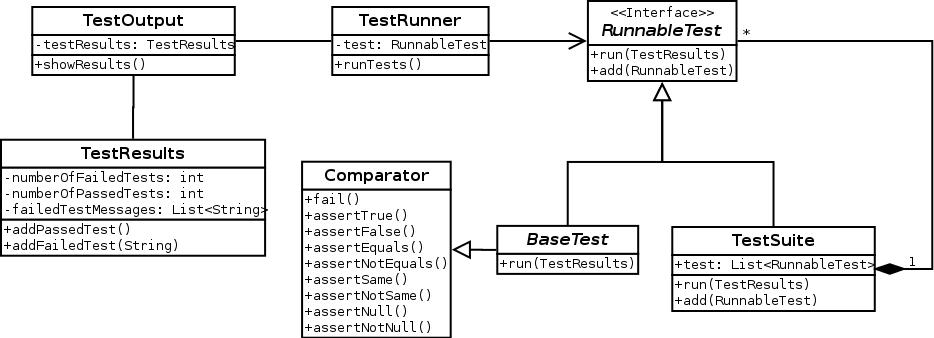
\includegraphics[scale=0.50,angle=90]{./ClassDiagram}
\end{center}
	\caption{diagrama de clases del trabajo práctico (entrega 1).}
\end{figure}

\subsection{Responsabilidades de las clases}
Se describe a continuación la responsabilidad de cada clase:
\begin{itemize}
	\item \textbf{Assertion}: es la clase que implementa las aserciones.

	\item \textbf{TestCase}: es la encargada de correr cada test unitario.
		Las clases que hereden de ella implementarán el código que 
		ejecuta las pruebas. 
				
	\item \textbf{TestContext}: esta clase contiene las instancias creadas
		por los usuarios a la hora de hacer setUps, y es utilizada
		a lo largo de toda la ejecución.
		
	\item \textbf{TextInformation}: es clase introducida para 
		encapsular la información de los test corridos anteriormente,
		los filtros de ejecución del usuario y la instancia de TestLogger
		para guardar los resultados.
		
	\item \textbf{TestLogger}: es la clase que desacopla a los tests en sí de
		las salidas que se usen para los resultados.
		
	\item \textbf{TestOutput}: es la encargada de interpretar los resultados
		y producir una salida legible.		
			
	\item \textbf{TestResults}: es una clase almacenadora de información
		sobre la ejecución de las pruebas.
	
	\item \textbf{TestRunner}: es el cliente en el esquema composite, crea
		una instancia de TestResults, ejecuta un TestSuite y luego
		muestra los resultados usando un TestOutput.	
		
	\item \textbf{TestSuite}: es la clase contenedora de todos los tests.
		Permite agregar tests y correrlos.

\end{itemize}

\section{Pruebas}
Se incluyen con la implementación varios sets de pruebas:

	\begin{enumerate}
	\item Pruebas unitarias: estas pruebas verifican el funcionamiento de 
	las clases desarrolladas usando jUnit 4. 
	
	Se intentó alcanzar una cobertura del 100\% del código con pruebas 
	unitarias, sin embargo se notó que había varias clases muy simples como 
	TestResult que probarlas pareció inútil.

	\item Pruebas de entorno: la intención de estas pruebas fue probar una 
	clase externa como lo haría el usuario.
	Se creo una clase con un comportamiento trivial y se generaron casos de
	prueba para después correrlos. 
	
	Se insertaron tanto pruebas que corren correctamente como pruebas que
	fallan, de manera de mostrar el funcionamiento completo del entorno.
	
	El mismo de set de pruebas se corrió con jUnit 4 para mostrar que 
	efectivamente los resultados obtenidos son equivalentes.
		\begin{enumerate}
		\item Pruebas de comparación: que verifican que funcione 
		correctamente las aserciones del framework ante diferentes 
		situaciones.
		\item Pruebas de anidación: que verifican que se ejecuten todos
		los casos de prueba en una corrida, anidando varios niveles
		de suites con casos.
		\item Pruebas de expresiones regulares: que verifican que se
		respete que sólo se corran aquéllas pruebas que cumplan con
		la expresión regular indicada.
		\item Pruebas de fixture: que verifican que se respeten los setUps
		y los tearDowns que corresponden para cada corrida.
		\end{enumerate}
	\end{enumerate}
	
\section{Conclusiones}
Durante el desarrollo del trabajo pudimos aplicar los conceptos adquiridos a lo
largo de la materia para hacer un código más mantenible, más legible y más
estandarizado que el que hubiéramos escrito antes de cursar.

Pudimos verificar que el diseño que implementamos en la primera entrega estaba
abierto a modificaciones y cerrado ante cambios porque las extensiones de los
requerimientos las pudimos hacer casi sin tocar código existente.

También hicimos uso extensivo de las herramientas que nos ofrece el IDE según lo
visto en las clases prácticas, como por ejemplo a la hora de refactorizar.

Finalmente pudimos apreciar las ventajas de tener desde el primer momento un set
de pruebas confiable, pues pudimos estar seguros en todo momento de que las 
modificaciones que introducíamos no hacían que código antiguo dejara de funcionar.

\end{document}
